LROSE (Lidar Radar Open Software Environment) là một dự án được Hỗ trợ bởi Quỹ Khoa học Quốc gia (NSF) với mục tiêu phát triển phần mềm chung cho cộng đồng Lidar, Radar và Profiler. Dự án hoạt động dựa trên nguyên tắc phát triển cộng tác và mã nguồn mở. Gói phần mềm cốt lõi của LROSE là sự hợp tác chung giữa Đại học Colorado (CSU) và Phòng thí nghiệm Quan sát Trái đất (EOL) tại Trung tâm Nghiên cứu Khí tượng Quốc gia (NCAR) \cite{lrose}.

LROSE xuất phát từ nhu cầu có một môi trường phần mềm thống nhất cho việc xử lý dữ liệu Lidar và Radar trong nghiên cứu khoa học về khí tượng học \cite{lrose}.
Dự án giải quyết những phức tạp liên quan đến việc tích hợp dữ liệu từ nhiều nền tảng quan sát khác nhau, bao gồm Lidar, Radar và Profiler. Các thành phần này được thiết kế để đáp ứng những nhu cầu cụ thể của các nhà khoa học khí tượng và nghiên cứu viên làm việc với dữ liệu cảm biến từ xa.

LROSE được sử dụng rộng rãi trong nghiên cứu khí tượng, bao gồm các nghiên cứu liên quan đến quá trình mây và mưa, động lực lớp biên, và các hiện tượng khí tượng khác. Phần mềm hỗ trợ phân tích dữ liệu quan sát thu thập từ các công cụ đặt trên mặt đất như Lidar và Radar. LROSE thường kết hợp mượt mà với đa dạng công cụ mô hình và phân tích khí tượng để tối ưu hóa khả năng của nó.Những nhà nghiên cứu thường tích hợp LROSE vào mô hình dự báo thời tiết số cũng như các kỹ thuật hòa nhập dữ liệu khác, tạo nên một hệ thống linh hoạt và mạnh mẽ.

\begin{figure}[H]
    \centering
    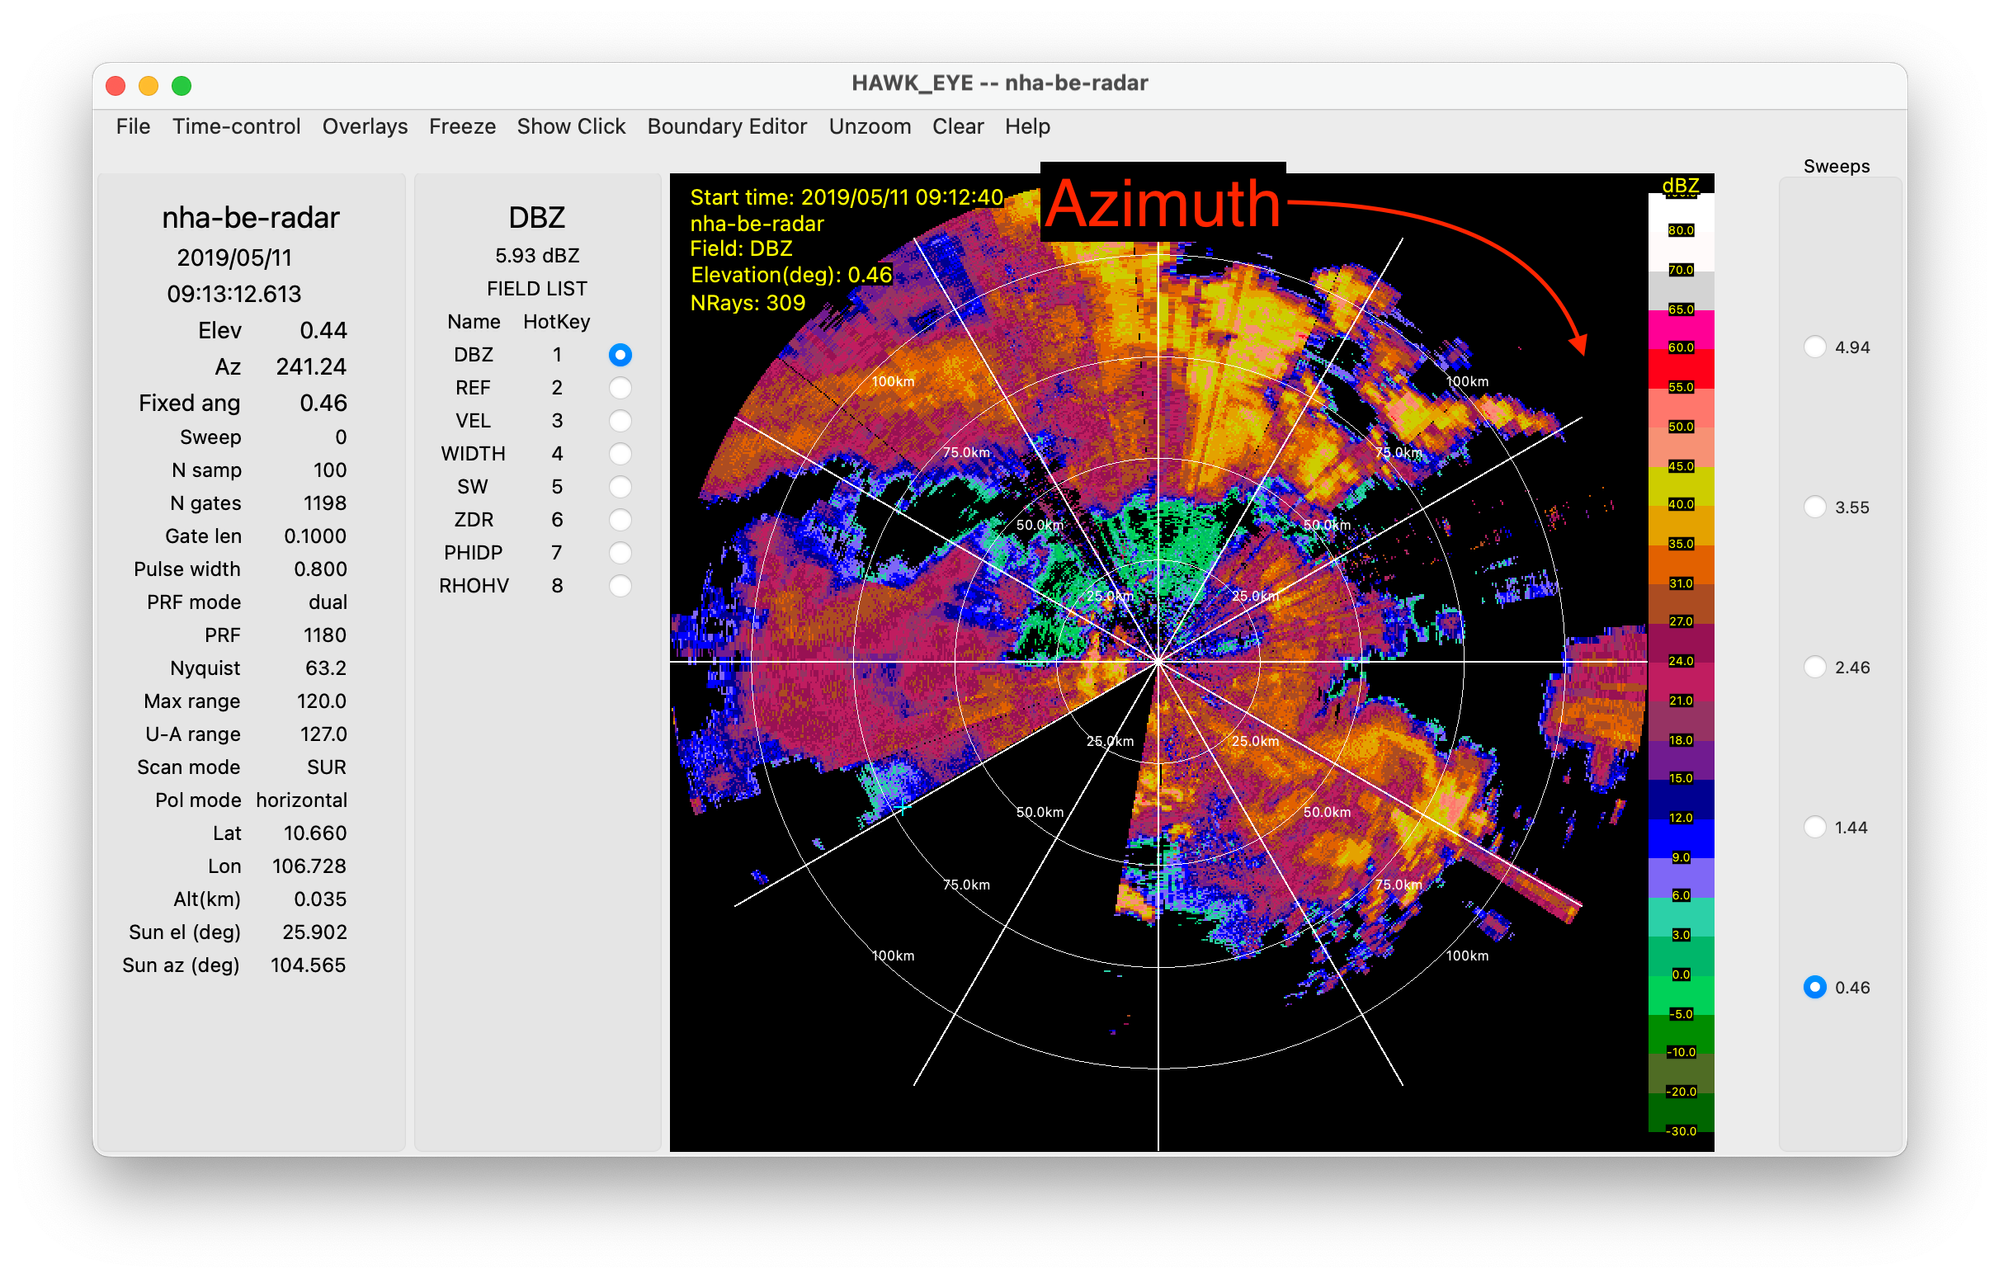
\includegraphics[width=0.8\linewidth]{Images/3.5-hawk-eye.png}
    \caption{Hawk Eye, Công cụ hiển thị lidar và radar của LROSE}
    \label{fig:hawk-eye}
\end{figure}

Dự án tích cực khuyến khích sự tham gia từ cộng đồng khoa học rộng lớn, thúc đẩy sự trao đổi ý kiến, thuật toán và cải tiến cho phần mềm.
Các cập nhật đều đặn và đóng góp từ người dùng góp phần vào quá trình phát triển và hoàn thiện liên tục của LROSE.